\chapter{城乡人口结构}
\label{chapter:people}

下图展示了全球人口结构随年复合增长率变化的情况。从图中可以得出两个主要观察结果:首先,全球发达国家的年复合增长率接近于零,而发展中国家的年复合增长率通常在1至3之间,非洲等不发达国家的年复合增长率则常超过5\%且波动较大。其次,像中国这样的发展中国家在图中显示为深绿色,与发达国家形成对比,显示出其巨大的发展潜力和尚未稳定的人口结构比例。因此,发展农村地区成为当前的主要发展目标之一。

\begin{figure}[H]
    \centering
    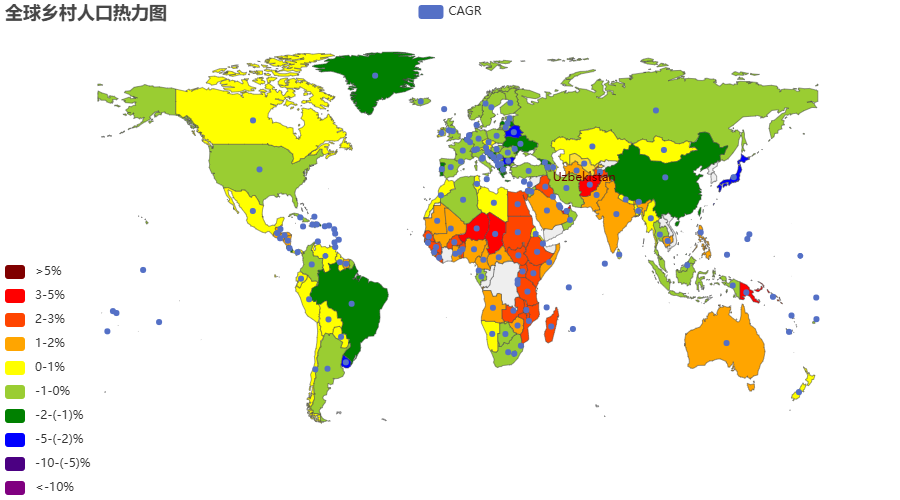
\includegraphics[width=1\linewidth]{pictures/image.png}
    \caption{全球乡村人口热力图}
    \label{fig:enter-label}
\end{figure}



自改革开放以来,中国农村面临着劳动力向城市大量流动的现象,这一趋势引发了乡村人口老龄化、劳动力流失等问题。为应对这些挑战,国家提出乡村振兴战略,旨在通过提高农业效率、改善基础设施和公共服务,以此来提升农村生活水平,从而促进农村经济社会全面发展。

随着乡村振兴战略的实施,乡村人口结构出现新变化。我们将利用1990年至2022年间每隔七年的数据,绘制一系列饼图来展示中国城镇人口和乡村人口的比例。

\begin{figure}[H]
    \centering
    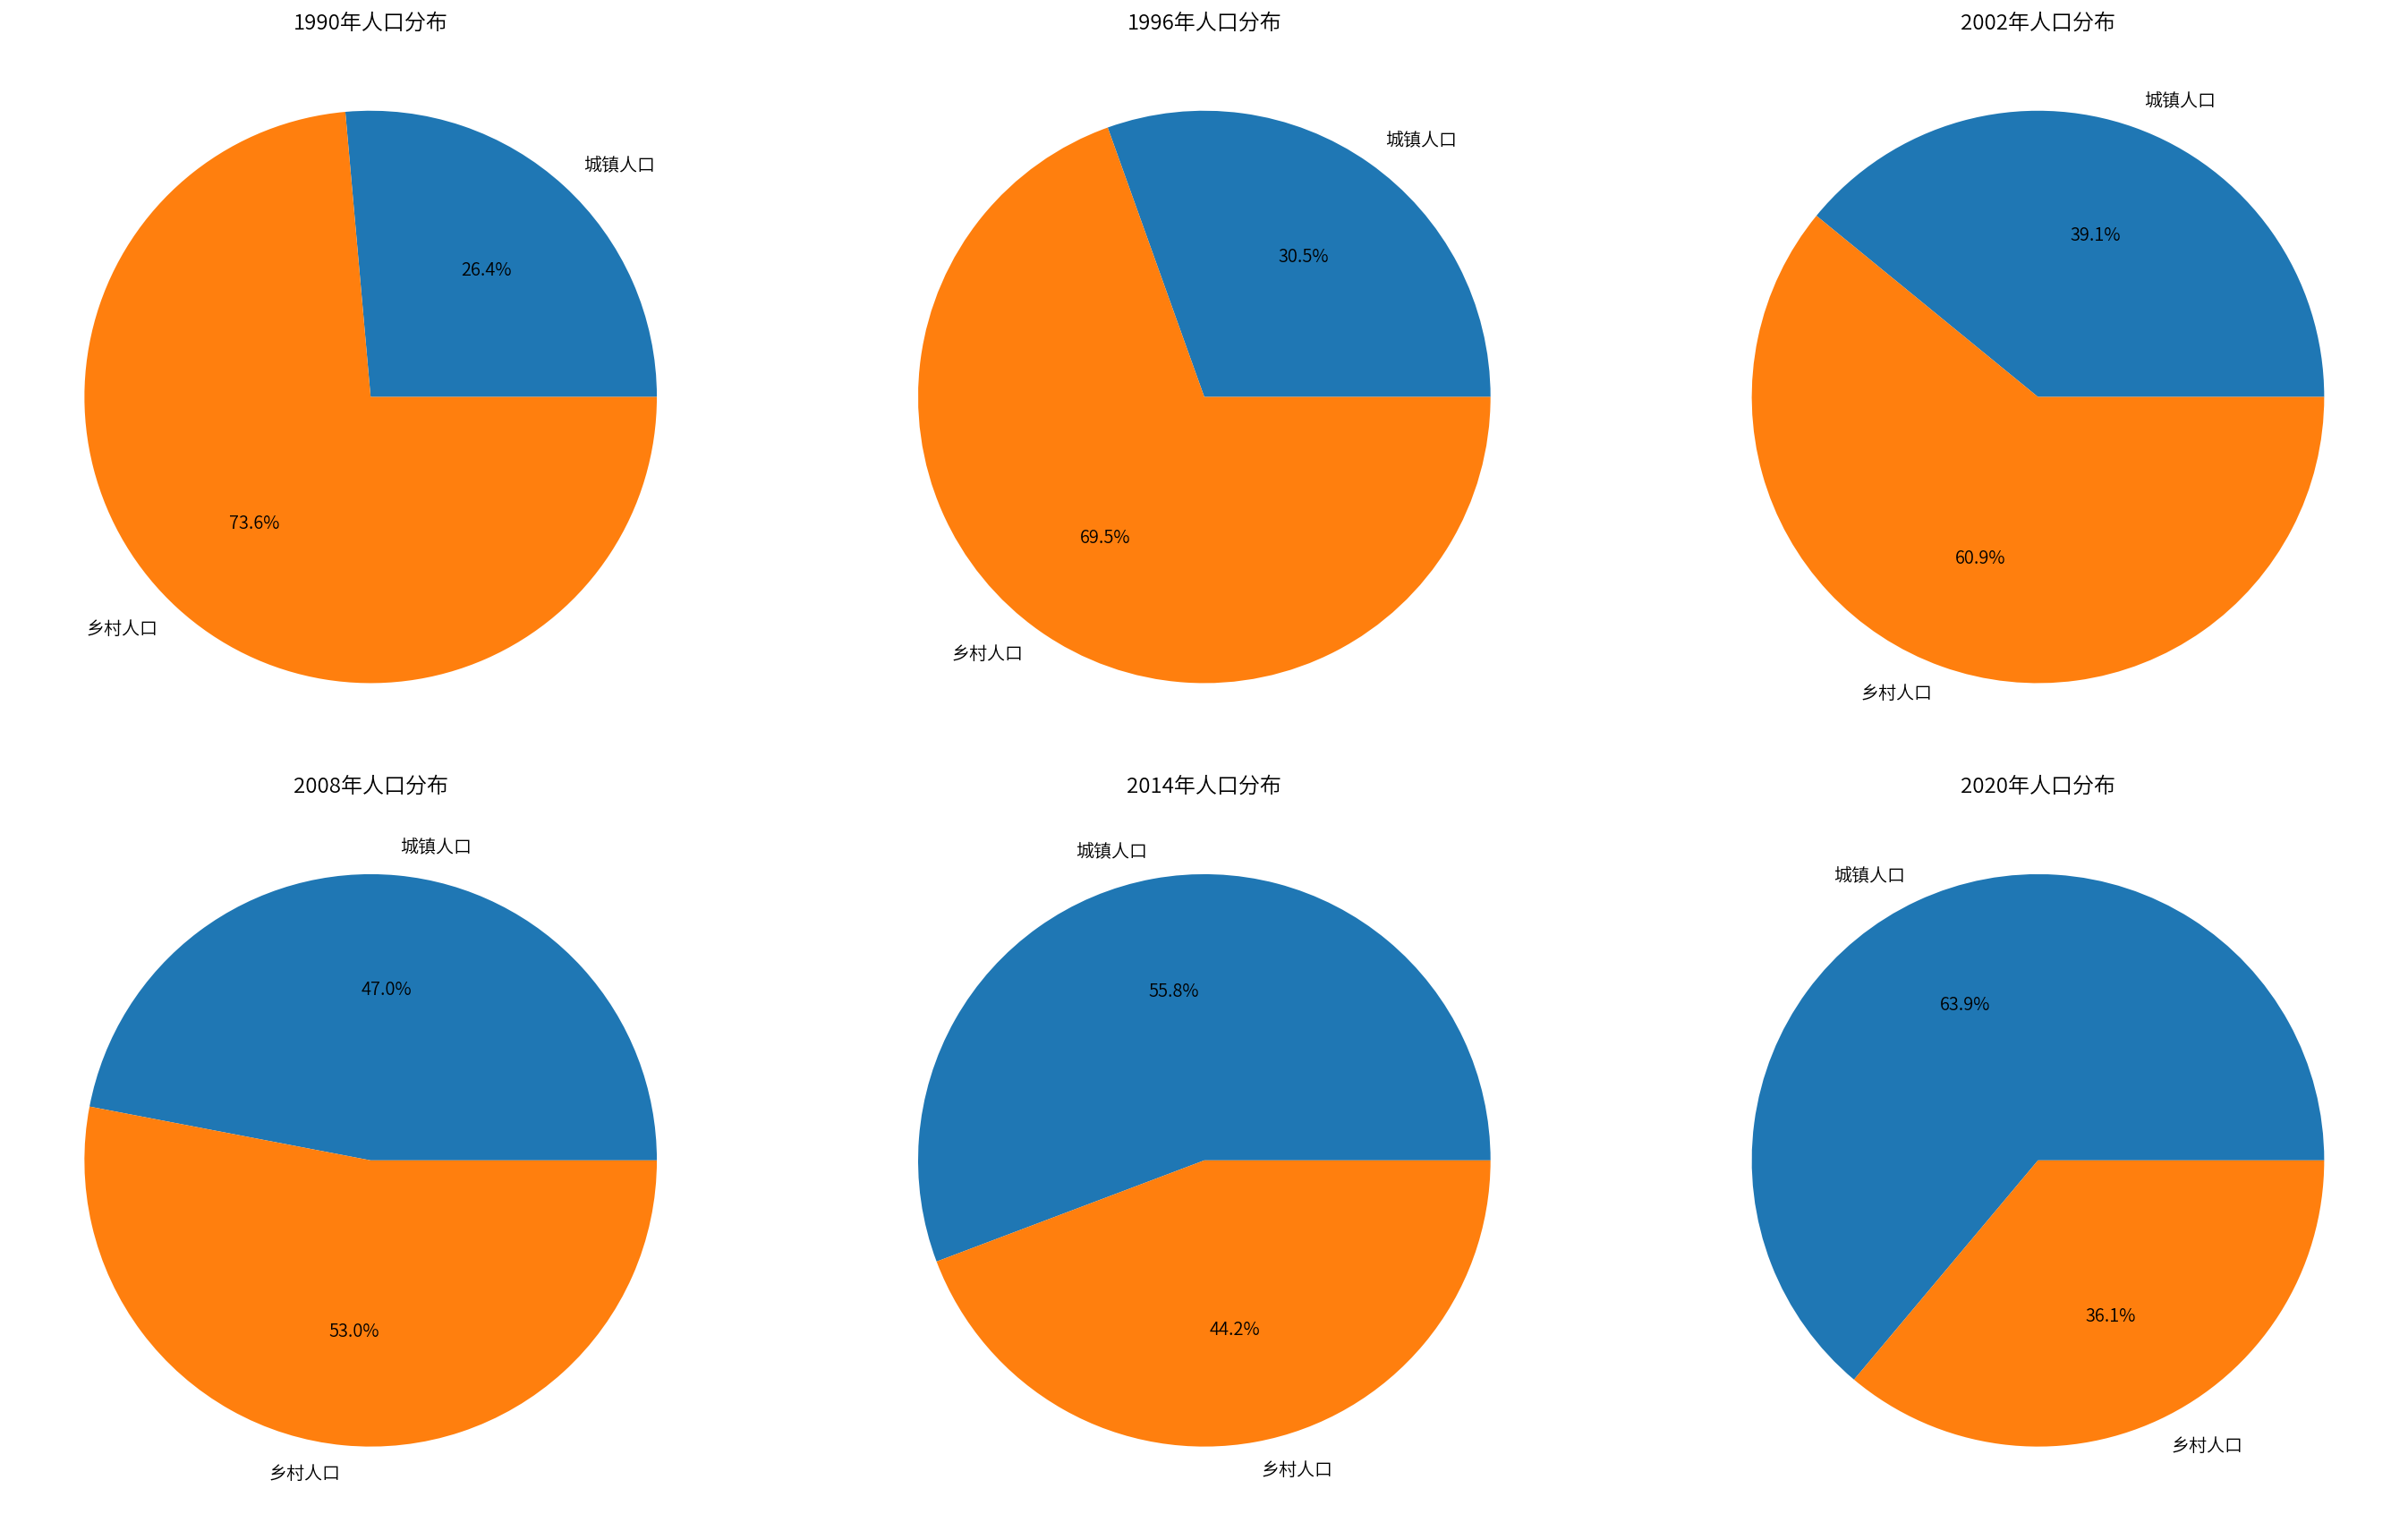
\includegraphics[width=1\linewidth]{figures/1.png}
    \caption{城乡人口占比图}
    \label{fig:city_village_population}
\end{figure}

图表显示,城镇人口占比逐年上升,而乡村人口占比相应地逐年下降。这一趋势与改革开放以来中国城市化进程的加快密切相关。

% 随着中国经济的快速发展、就业机会的增多以及城市生活条件的持续改善,大量农村居民被吸引到城市中寻求更好的工作和生活机会。这一趋势导致城市人口比重逐年攀升,而乡村人口比重相应地逐年下降。这种人口流动不仅反映了城乡之间的经济差距,也揭示了农村地区在发展机会、基础设施、教育、医疗等方面的不足。

农村地区的人口流失进一步凸显了农村发展的迫切需求。为了缓解这一趋势,必须加强农村建设和政策吸引,提供更多的就业机会,改善教育和医疗条件,以及提高农民的生活水平,为农村居民创造更有吸引力的生活和工作环境,减缓乡村人口的流失速度,促进城乡协调发展。正是在这样的历史背景下,乡村振兴战略应运而生,成为了中国特色社会主义新时代的重要篇章。

\section{城乡人口预测}
进一步分析发现,尽管乡村人口比例持续下降,但下降的速度似乎在放缓,显示出比例减少的幅度逐渐减小。这可能反映了近年来中国在推进城乡发展一体化、实施乡村振兴战略等方面所做的努力开始显现成效,乡村人口流失速度有所放缓。

为了验证城乡人口变化趋势的猜想并预测未来发展,本文采用了DLF-LSTM模型预测接下来五年内城乡人口的变化趋势。所得到的预测结果以及模型对历史数据的拟合情况通过下图展示。
\begin{figure}[H]
    \centering
    \begin{minipage}{0.5\textwidth}
        \centering
        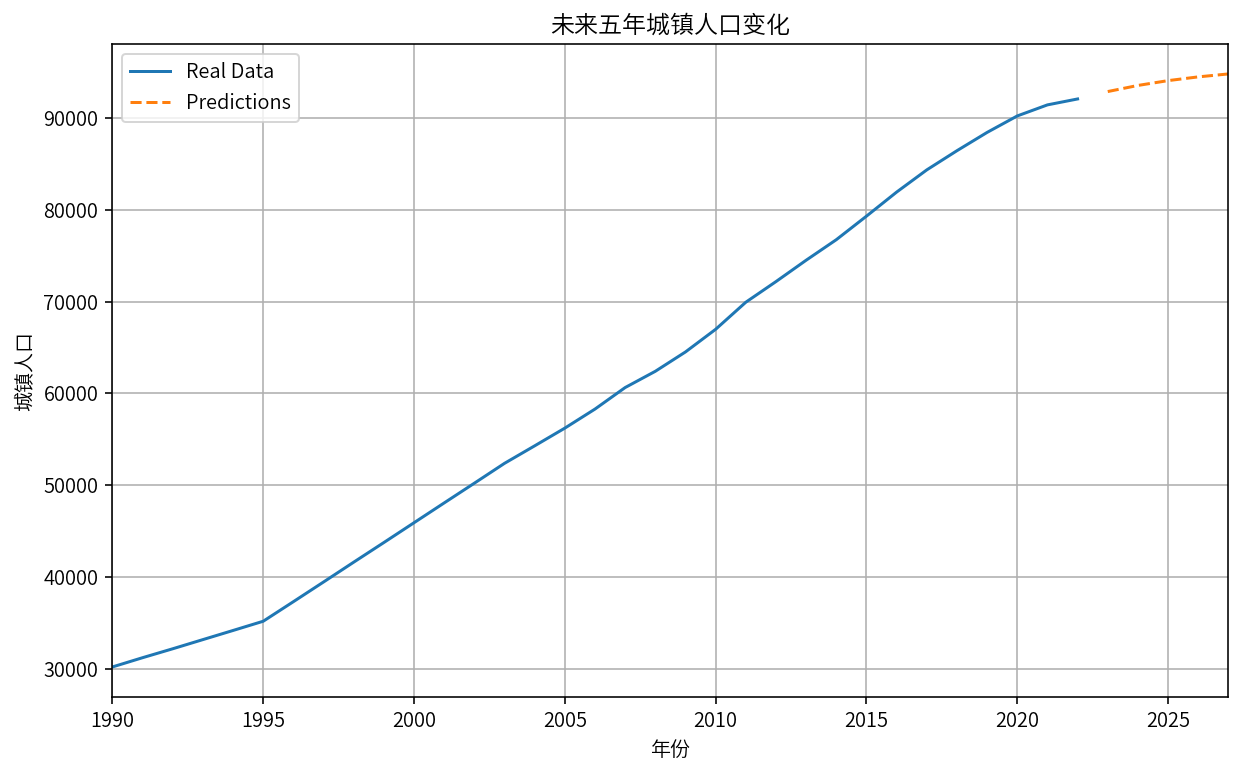
\includegraphics[width=\linewidth]{figures/2.png}
        \caption{未来五年城镇人口变化}
        \label{fig:population-change}
    \end{minipage}\hfill
    \begin{minipage}{0.5\textwidth}
        \centering
        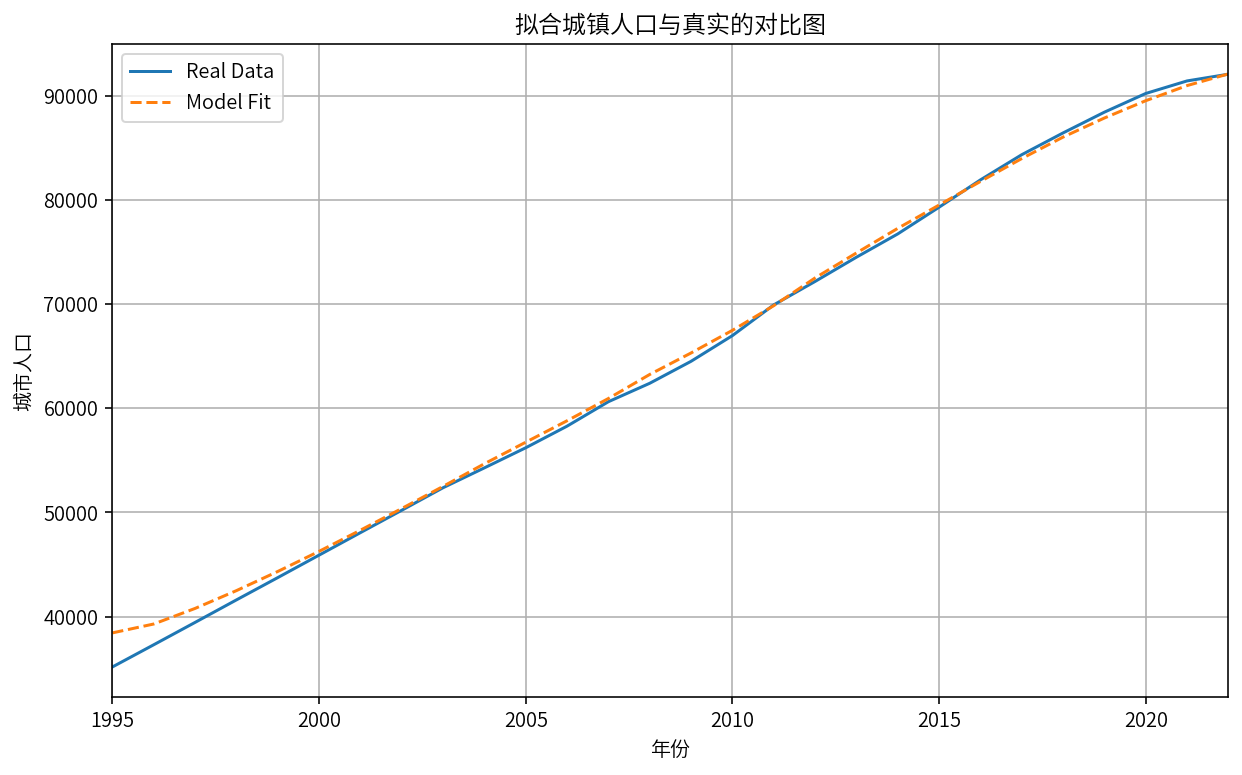
\includegraphics[width=\linewidth]{figures/3.png}
        \caption{拟合城镇人口和真实的对比图}
        \label{fig:population_fit-vs-real}
    \end{minipage}
\end{figure}

通过时间序列得知,城镇后几年的趋势可能出现饱和,只有轻微的增长。

接着同样方法分析农村人口的预测,所得结果如下:
\begin{figure}[H]
    \centering
    \begin{subfigure}{0.5\textwidth}
        \centering
        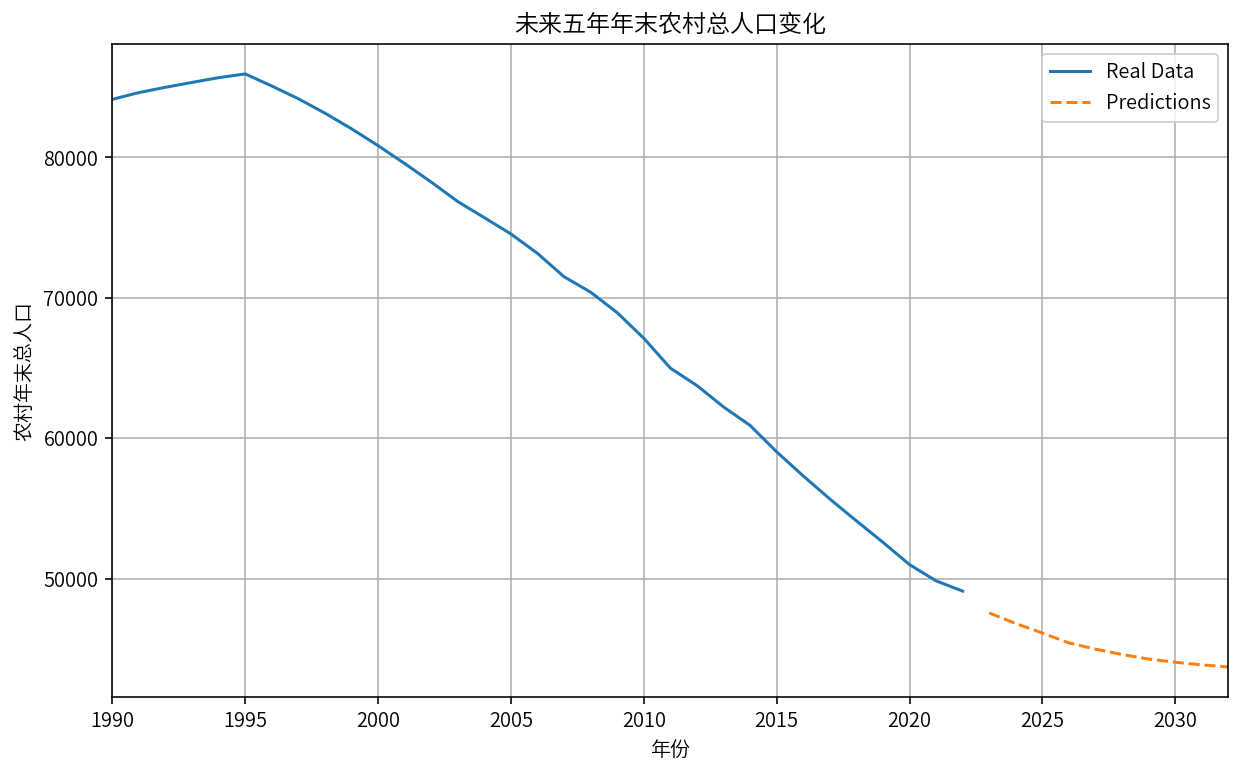
\includegraphics[width=\linewidth]{figures/35.png}
        \caption{未来五年农村人口变化}
        \label{fig:sub1}
    \end{subfigure}%
    \begin{subfigure}{0.5\textwidth}
        \centering
        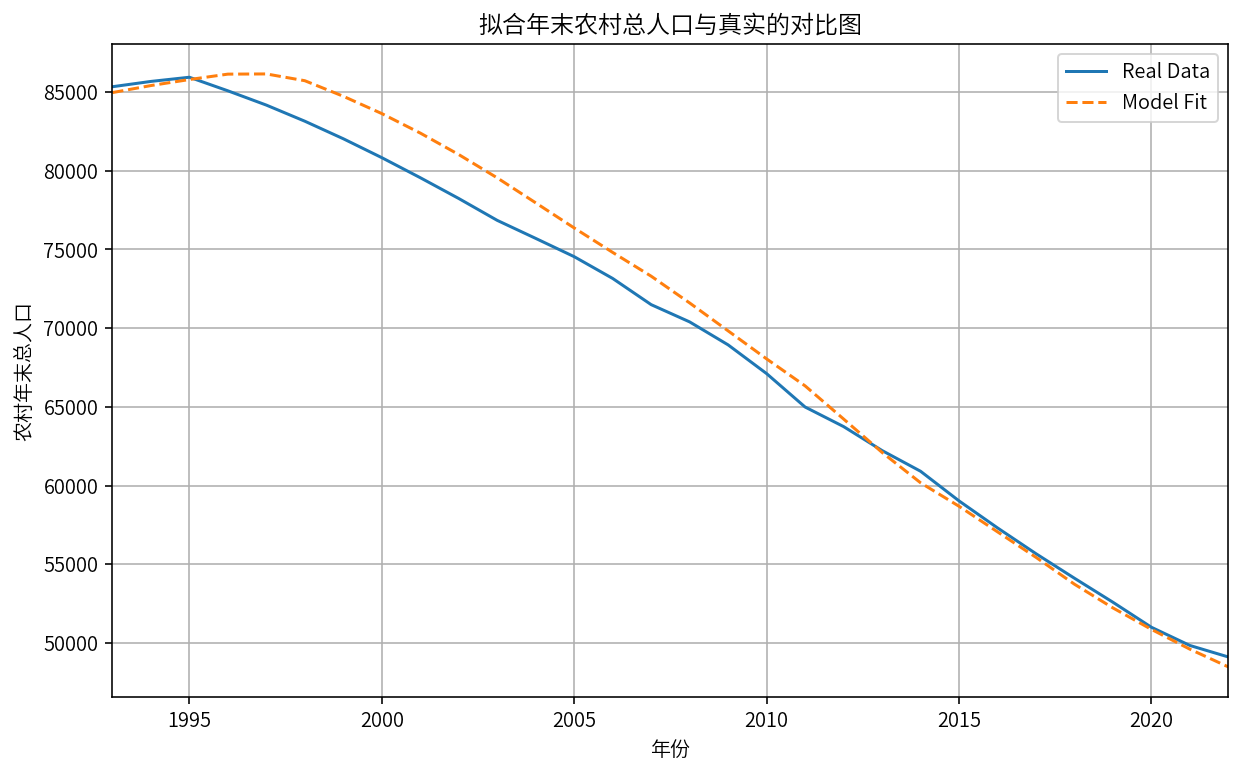
\includegraphics[width=\linewidth]{figures/36.png}
        \caption{拟合农村人口和真实的对比图}
        \label{fig:sub2}
    \end{subfigure}
    \caption{农村人口变化图}
    \label{fig:combined}
\end{figure}

\begin{table}[h]
    \centering
    \begin{minipage}{0.48\linewidth}
        \centering
        \caption{未来城镇人口预测}
        \label{tab:urban_population_prediction}
        \begin{tabular}{cc}
        \hline
        年份 & 预测城镇人口(万人) \\
        \hline
        2023 & 92876.58 \\
        2024 & 93542.80 \\
        2025 & 94068.30 \\
        2026 & 94475.73 \\
        \hline
        \end{tabular}
    \end{minipage}\hfill
    \begin{minipage}{0.48\linewidth}
        \centering
        \caption{未来农村总人口预测}
        \label{tab:rural_population_prediction}
        \begin{tabular}{cc}
        \hline
        年份 & 预测农村总人口(万人) \\
        \hline
        2023 & 47548.48 \\
        2024 & 46795.32 \\
        2025 & 46118.73 \\
        2026 & 45412.10 \\
        \hline
        \end{tabular}
    \end{minipage}
\end{table}



随后,本文对每年农村人口变化与前一年的比例进行了汇总,并比较了其与1的大小。当这个比例接近1时,说明农村人口的减少趋势相对较小,而当这个比例远离1时,则意味着变化幅度较大。

\begin{figure}[H]
    \centering
    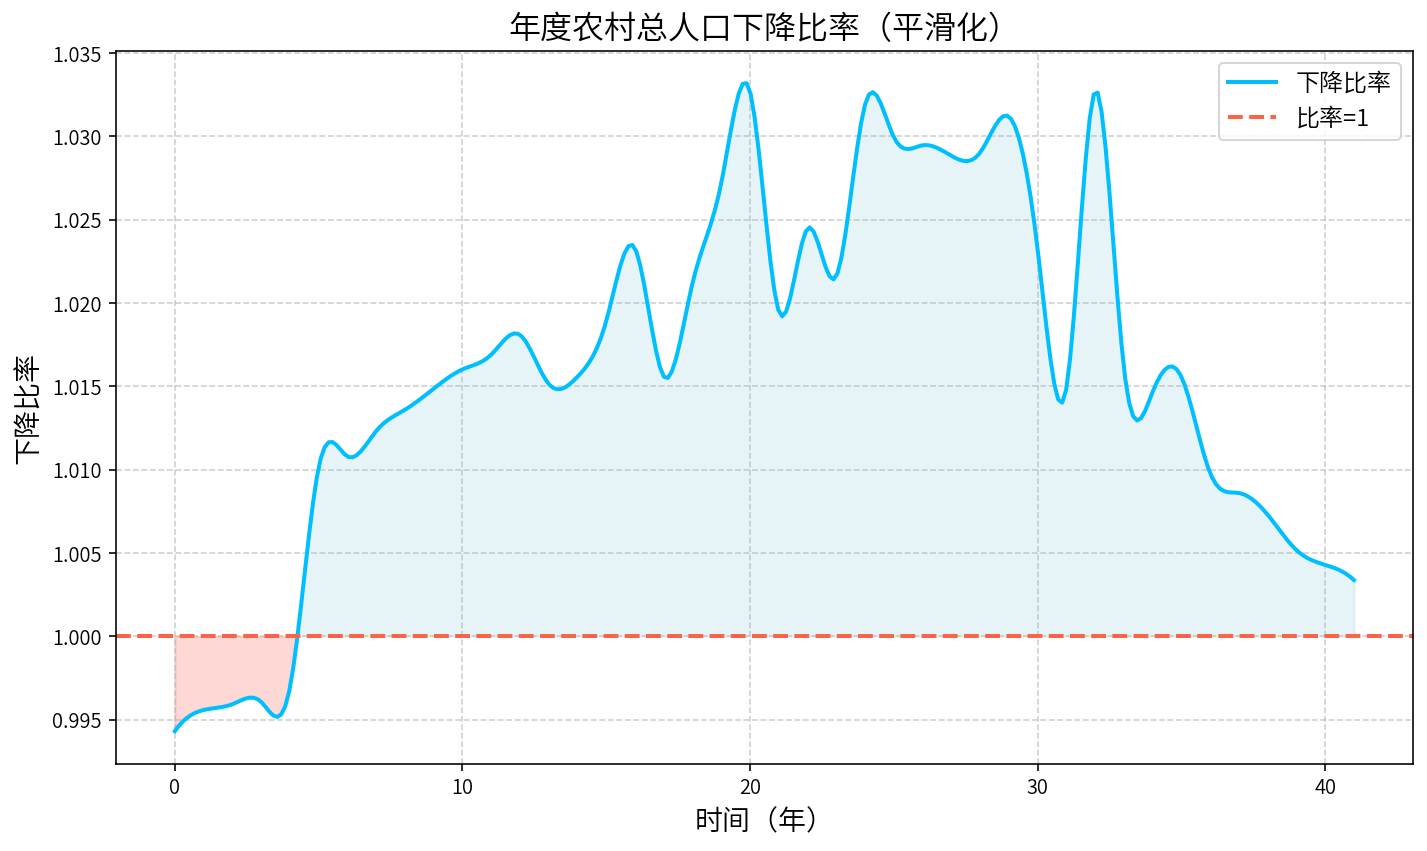
\includegraphics[width=0.65\linewidth]{figures/37.png}
    \caption{年度农村总人口下降比率}
    \label{fig:enter-label}
\end{figure}
三者的结果均显示,农村人口未来的变化趋势或许会受到乡村振兴政策的积极影响,呈现出逐渐趋于平缓甚至可能有所增加的态势。这暗示着在未来一段时间内,农村地区可能会迎来一定程度的人口回流,这可能是乡村振兴战略所带来的积极结果。

这一战略不仅是对中国农村问题的深刻反思,更是对实现城乡和谐发展愿景的坚定追求。在此战略下,农业不再是单一的粮食生产,而是转型为现代化、多元化的产业体系。农村不再是落后的代名词,而是成为充满活力和希望的土地。农民不再是时代的边缘人,而是成为享受现代文明成果的主体。

% 一方面,一些地区通过改善农村生活环境和提高农业产业的吸引力,成功吸引部分人口返乡创业或回归农业,逐渐形成了城乡人口流动的双向互动模式。另一方面,随着农村教育、医疗和生活条件的改善,农村居民的生活质量逐步提升,农村地区的人口外流压力有所缓解,乡村社区开始呈现出更加活力和可持续发展的态势。这些变化反映了乡村振兴战略在调整人口结构、促进城乡均衡发展方面的积极成效。

